\documentclass{article}
\usepackage{indentfirst}
\usepackage{graphicx}
\usepackage{mathtools}
\usepackage{float}
\usepackage{hyperref}
\hypersetup{
    colorlinks,
    citecolor=black,
    filecolor=black,
    linkcolor=black,
    urlcolor=black
}

\graphicspath{ {.} }
\renewcommand{\figurename}{Obrázek}

\begin{document}

\title{Poznámky ke stáži}
\author{Matěj Gajdoš}

\maketitle
\newpage
\tableofcontents
\newpage

\section{Metastabilní Isingův model}
\subsection{Dynamika}
Nechť $\Lambda$ je mřížka, $i$ je uzel $\Lambda$, $x = (x_1, x_2)$ je stochastický proces na $\Lambda$ se stavovým prostorem $S = \{-1; 1\} \times \{-1; 1\}$, $F_k(i)$ je počet uzlů $j$ sousedících s $i$, pro které platí $x_k(j) = x_k(i)$. Zároveň pro $j \in \Lambda$

\begin{equation}
    R_1(j) = 
    \begin{cases*}
      1 & pokud $x_1(j) = x_2(j)$ \\
      0        & jinak
    \end{cases*}
\end{equation}
\begin{equation}
    R_2(j) = 
    \begin{cases*}
      1 & pokud $x_1(j) \neq x_2(j)$ \\
      0        & jinak
    \end{cases*}
\end{equation}

Pak je dynamika Metastabilního Isingova modelu následující: Nejdříve se vybere uzel $i \in \Lambda$ a $k \in \{1; 2\}$ uniformě náhodně. Následně se s mírou $\exp(-\beta F_k(i) - \alpha R_k(i))$ otočí hodnota procesu $x_k$ v uzlu $i$, $x'_k(i) = -x_k(i)$.

Proces $x_1$ budeme dále označovat jako proces $X$ a proces $x_2$ jako $Y$. 

\subsection{Prostorová mřížka}
Ze simulací na konečné prostorové kubické mřížce, jejíž koncové uzly jsou propojeny, se zdá, že pro vhodné $L, \alpha$ a $\beta$ systém vykazuje globální periodické chování. Výpočetní náročnost simulací ale se vzrůstajícím $L$ rychle roste, tudíž lze prakticky simulovat pouze systémy s relativně malým $L$.
\subsubsection{Fázový diagram}
V závislosti na volbě parametrů $\alpha$ a $\beta$ se simulace modelu mohou chovat minimálně čtyřmi způsoby. Fáze je určena na základě celkové střední hodnoty systému $E$ a střední hodnoty amplitudy $E[A]$, přičemž amplitudy korespondují s časovým průběhem střední hodnoty mřížky, E($t$). Zatím simulace proběhly pro $\alpha \in \left[ -3.5; 3.5 \right], \beta \in \left[ 0; 12 \right]$.

Při hodnotách $\beta \rightarrow 0$ systém nevykazuje žádné globální chování. Pro vhodné kombinace $\alpha$ a $\beta$ se systém chová periodicky, příčemž pro dané $\alpha$ platí, že s rostoucím $\beta$ roste i periodičnost systému ve smyslu vyšších amplitud v grafu E($t$). Pro $\beta >> \alpha$ se systém stabilizuje a všechny uzly mřížky nabývají jedné hodnoty. Pro $\beta < 0$ se systém také může stabilizovat, ale v takovém případě připomíná Antiferromagnetický Isingův model.

V obrázcích vývoje mřížky jsou pro různé parametry zvoleny různé časové intervaly. Je tomu tak, protože "rychlost plynutí času" (ve smyslu toho, jak dlouho obvykle trvá, než se nějaký uzel změní) závisí na parametrech $\alpha$ a $\beta$. Proto bylo pro všechny simulace, ke kterým se obrázky vztahují, zvoleno, že se mají zastavit po $10^6$ změnách, protože pokud by byl namísto toho určen maximální čas, pak by některé simulace trvaly příliš dlouho, a jiné by nemusely stihnout dosáhnout svého charakteristického chování. 

\begin{figure}[H]
    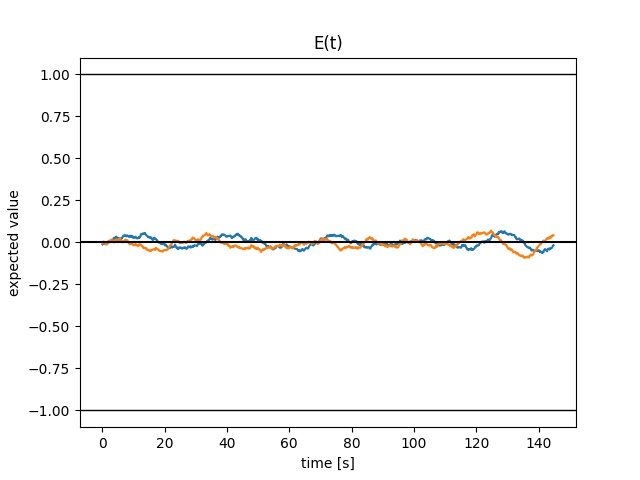
\includegraphics[scale=0.8]{A1B2L20_graph}
    \caption{Střední hodnoty dvou procesů v závislosti na čase pro $\alpha = 1, \beta = 2, L = 20$}
\end{figure}
\begin{figure}[H]
    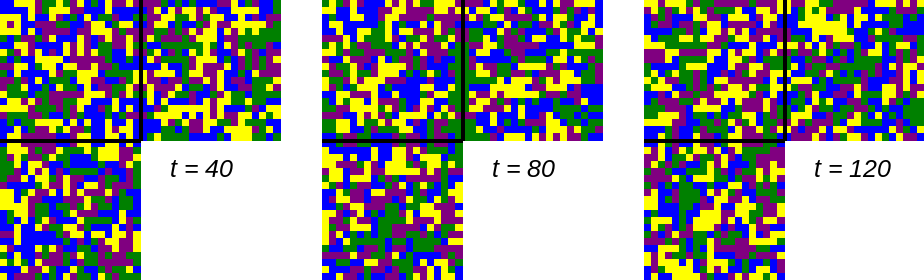
\includegraphics[scale=0.4]{A1B2L20_evolution}
    \caption{Vývoj systému s $\alpha = 1, \beta = 2, L = 20$}
\end{figure}

\begin{figure}[H]
    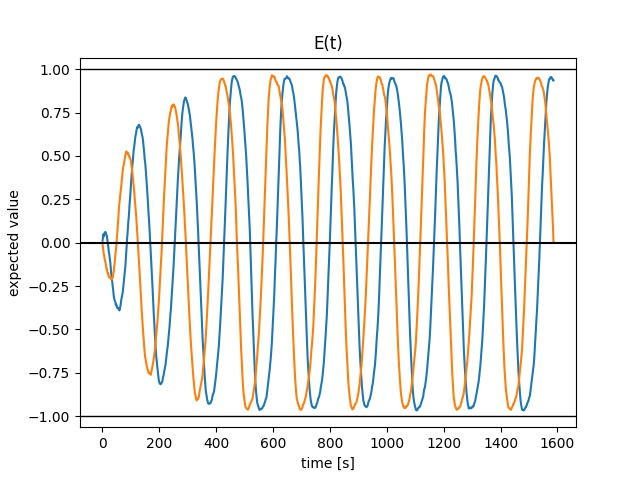
\includegraphics[scale=0.8]{A1B4L20_graph}
    \caption{Střední hodnoty dvou procesů v závislosti na čase pro $\alpha = 1, \beta = 4, L = 20$}
\end{figure}
\begin{figure}[H]
    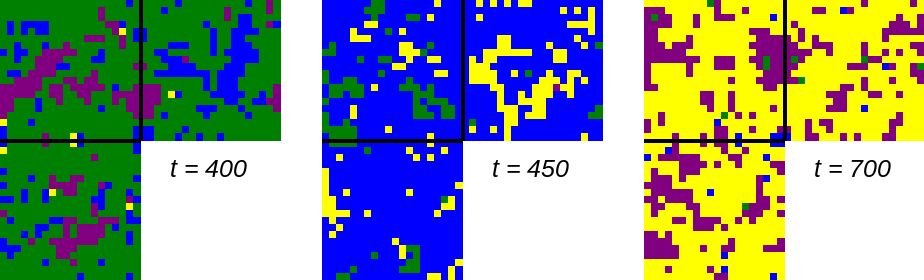
\includegraphics[scale=0.4]{A1B4L20_evolution}
    \caption{Vývoj systému s $\alpha = 1, \beta = 4, L = 20$}
\end{figure}

\begin{figure}[H]
    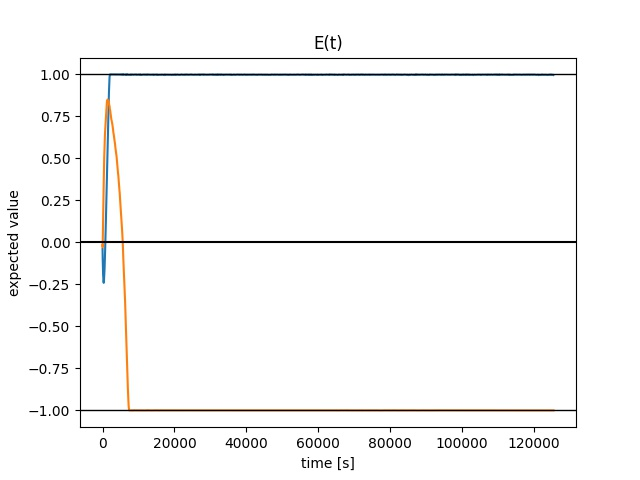
\includegraphics[scale=0.8]{A1B8L20_graph}
    \caption{Střední hodnoty dvou procesů v závislosti na čase pro $\alpha = 1, \beta = 8, L = 20$}
\end{figure}
\begin{figure}[H]
    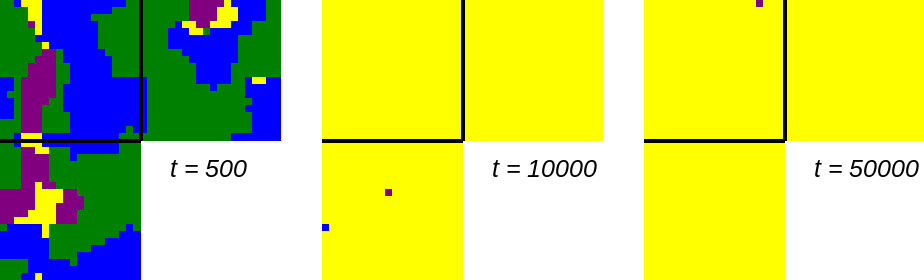
\includegraphics[scale=0.4]{A1B8L20_evolution}
    \caption{Vývoj systému s $\alpha = 1, \beta = 8, L = 20$}
\end{figure}

\begin{figure}[H]
 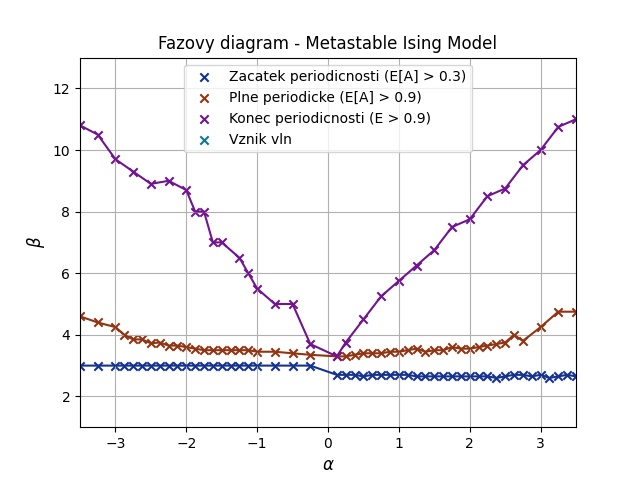
\includegraphics{phase_diagram}
 \caption{Fázový diagram Metastabilního Isingova modelu.}
 \label{fig:phase_diagram}
\end{figure}

\subsection{Perioda}
Pokud systém vykazuje periodické chování, můžeme mu přiřadit periodu pomocí grafu střední hodnoty mřížky v závislosti na čase. Graf závislosti periody na parametru $\beta$ pro konstantní $\alpha = 2$ lze vidět níže.

\begin{figure}[H]
 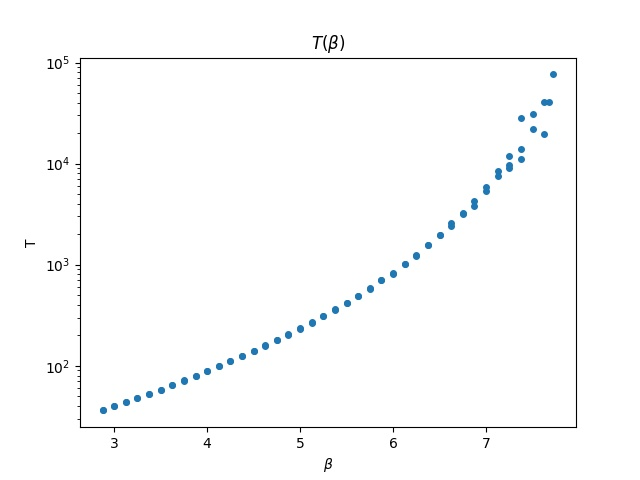
\includegraphics{T_beta_only}
 \caption{Závislost periody $T$ na parametru $\beta$ pro $\alpha = 2$ (svislá osa v logaritmické škále).}
 \label{fig:T_beta_only}
\end{figure}

Z Obrázku~\ref{fig:T_beta_only} je patrné, že na intervalu $(7.5,8)$ začíná být mezi body se stejným $\beta$ větší rozptyl v souřadnici $T$ a že funkce rychleji roste. Z fázového diagramu (viz Obrázek~\ref{fig:phase_diagram}) lze vyčíst, že někde v tomto intervalu byl ze simulací zachycen přechod mezi periodickou fází a konstantní, "zamrzlou" fází. Není ale úplně zřejmé, jestli se systém opravdu přestane chovat periodicky, nebo je jen perioda příliš velká pro zachycení ve standardních simulacích. Pokud by opravdu docházelo ke změně fáze a ztrátě periodičnosti, mohla by funkce $T(\beta)$ mít někde na intervalu $(7.5, 8)$ (pro $\alpha = 2$) asymptotu - viz Obrázek~\ref{fig:T_beta_fit}, kde byly body proloženy křivkou s asymptotou v $7.8$.

\begin{figure}[H]
 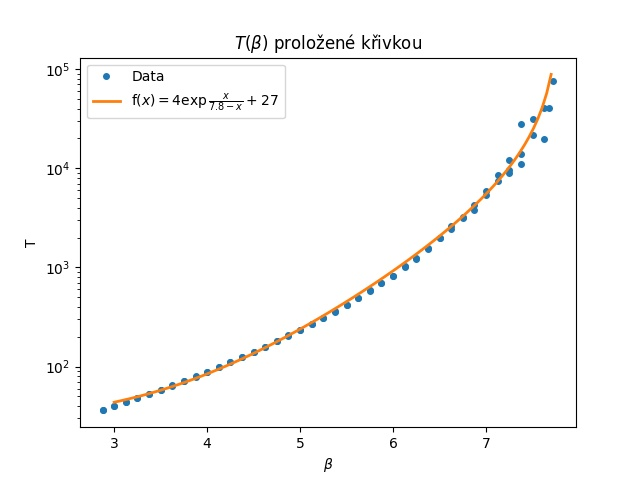
\includegraphics{T_beta_fit}
 \caption{Závislost periody $T$ na parametru $\beta$ pro $\alpha = 2$ (svislá osa v logaritmické škále). Body jsou proloženy křivkou funkce $f(\beta)$, která má asymptotu v $7.8$.}
 \label{fig:T_beta_fit}
\end{figure}


\subsection{Vlny}
Vývoj systému může připomínat vlnění, tedy jedním směrem se šířící změna stavu. Pro $\beta > 0$ zatím nebyl zaznamenán případ, kdy by vlny spontánně vznikaly, ovšem pro určité kombinace $L, \alpha$ a $\beta < 0$ ano. Konkrétní kombinace těchto parametrů, při nichž se systém vlní, a relativní četnost jejich vzniku je ještě třeba blíže prozkoumat. Vlny lze uměle vyvolat vhodným počátečním rozdělením stavů na mřížce, takto vzniklé vlny jsou ale nejspíš méně stabilní než globální periodické chování mřížky, které bývá konečným stavem těchto simulací.
\begin{figure}[H]
 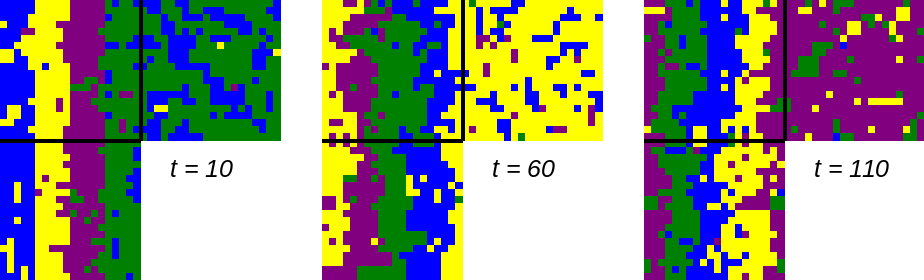
\includegraphics[scale=0.4]{induced_waves}
 \caption{Uměle vytvořené vlny pro $L = 20, \alpha = 1, \beta = 4$}
\end{figure}


\begin{figure}[H]
 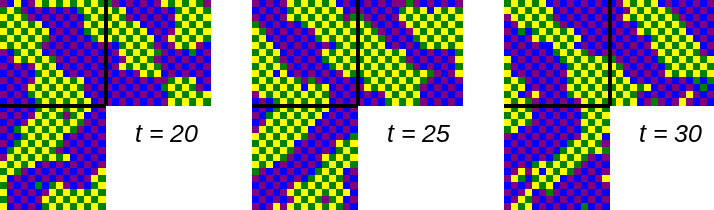
\includegraphics[scale=0.5]{spontaneous_waves}
 \caption{Spontánně vzniklé vlny pro $L = 15, \alpha = 2, \beta = -6$}
\end{figure}

\begin{figure}[H]
    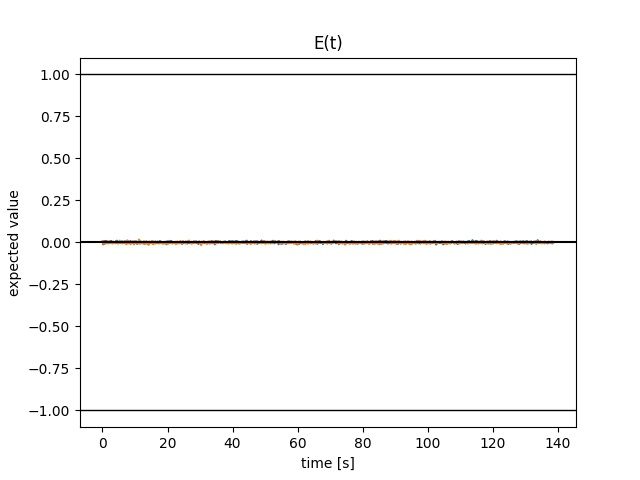
\includegraphics[scale=0.8]{spontaneous_waves_graph}
    \caption{Střední hodnoty dvou procesů v závislosti na čase pro $\alpha = 1, \beta = -6, L = 15$ (se spontánně vzniklými vlnami)}
\end{figure}

\subsubsection{Mechanismus propagace}
V Obrázku~\ref{fig:vlna_smer}, na němž je znázorněna vlna v rovině pro $\alpha = 2, \beta = -8$ a $L = 25$, jsou označeny oranžově uzly $i$, v nichž je v daném čase $T$ $Y_T(i) = 1$, naopak modře ty, v nichž je $Y_T(i) = -1$. Zároveň uzly $i$ v čase $T$, pro něž platí $X_T(i) = 1$, jsou světlejší, v opačném případě jsou tmavší.

\begin{center}
\begin{tabular}{ c|c|c|c }
 \textbf{X} & \textbf{Y} & \textbf{odstín} & \textbf{barva} \\ 
\hline
 1 & 1 & světlý & oranžová  \\  
 1 & -1 & světlý & modrá \\   
 -1 & 1 & tmavý & oranžová  \\  
 -1 & -1 & tmavý & modrá
\end{tabular}
\end{center}

V obrázku~\ref{fig:vlna_smer} jsou bíle a růžově vyznačeny rozhraní dvou oblastí. Uzly uvnitř těchto oblastí jsou relativně stabilní a pravděpodobnost jejich otočení je malá, tudíž nejvíce změn se dá očekávat právě v těchto rozhraních. Hlavní vliv má na vývoj v tomto případě $\beta$-interakce, protože $|\beta| > |\alpha|$. Uzly, které sousedí s větším počtem uzlů ze své oblasti než z druhé oblasti, si pravděpodobně svůj stav zachovají (např. pokud tmavě oranžový $(-1, 1)$ sousedí se třemi světle modrými $(1, -1)$ a jedním tmavě modrým $(-1, -1)$, pak si nejspíš svůj stav zachová). Hlavní změny tedy lze očekávat v uzlech z rozhraní, které mají stejně "svých" sousedů, jako těch opačných, protože tyto uzly nejsou stabilizovány $\beta$-interakcí.

\begin{figure}[H]
 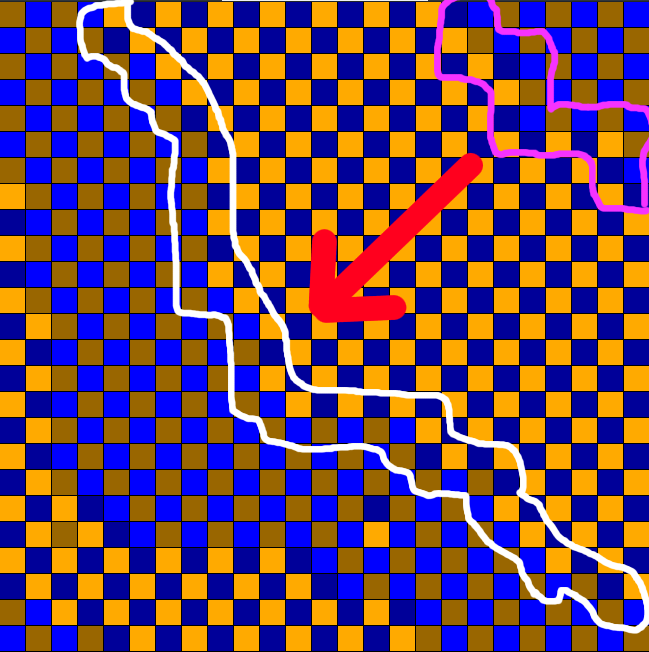
\includegraphics[scale=0.5]{vlna_smer}
 \caption{Směr šíření vlny určený z rozhraní oblastí; $\alpha = 2, \beta = -8, L = 25$}
 \label{fig:vlna_smer}
\end{figure}

V bílé oblasti vždy světle oranžový uzel sousedí se světle modrým uzlem a tmavě modrý uzel s tmavě oranžovým uzlem. Světle oranžový uzel odpovídá $(X, Y) = (1, 1)$ a světle modrý uzel $(X, Y) = (1, -1)$. Uvažujme situaci, kde světle oranžový uzel i světle modrý uzel mají stejný počet sousedů ze své oblasti jako těch z opačné oblasti (viz Obrázek~\ref{fig:detail_stabilita_vln}). Proces $Y$ je v tomto případě stabilní, protože oranžové uzly mají $Y = 1$, ty zde vždy sousedí s modrými uzly, které mají $Y = -1$, a míra otáčení je tedy (pro $\alpha = 2, \beta = -8$)

\[ \exp(-(-8)\cdot 0-2R_2) = \exp(-2R_2), R_2 \in \{0, 1\}, \]
což je shodné se stabilními uzly uvnitř oblastí.

Procesy $X$ se ale liší, a protože oba uzly mají polovinu sousedů z opačné oblasti, bude míra otáčení 

\[\exp(-(-8) \cdot 0.5 - 2R_1) = \exp(4 - 2R_1), R_1 \in \{0, 1\},\] 
tedy proces $X$ v těchto uzlech se bude často měnit, aniž by se stabilizoval. Protože ale v případě světle oranžového uzlu je $X = Y$, bude v tomto uzlu $R_1 = 1$, zatímco u světle modrého uzlu, kde $X \neq Y$, bude $R_1 = 0$, a tedy pro světle oranžový uzel je celková míra otáčení rovna $\exp(4 - 2 \cdot 1) = e^2$ a pro světle modrý uzel je míra otáčení $\exp(4 - 2 \cdot 0) = e^4$. Ke stejným výsledkům se dostaneme i při porovnání oblastí, kde sousedí tmavě modrý uzel s tmavě oranžovým uzlem. Důsledkem je, že v bílé oblasti jsou uzly z pravé oblasti (tmavě modré a světle oranžové) o něco stabilnější než ty v levé oblasti, a tedy se pravá oblast začne do levé oblasti šířit.


\begin{figure}[H]
 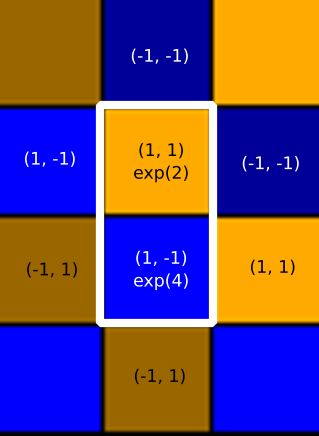
\includegraphics[scale=0.8]{detail_stabilita_vln}
 \caption{Detail situace dvou sousedících uzlů z rozhraní s jejich mírou otáčení pro $\alpha=2, \beta=-8$}
 \label{fig:detail_stabilita_vln}
\end{figure}

Naopak v uzlech z růžové oblasti je proces $X$ relativně stabilní, neboť spolu vždy sousedí dva různé odstíny, tudíž sousedící uzly $i, j$ mají $X(i) \neq X(j)$. Analogicky k bílému rozhraní je v růžovém rozhraní o něco stabilnější proces $Y$ z pravé oblasti než ten v levé - např. pro světle oranžovou $(1,1)$ a tmavě oranžovou $(-1,1)$ jsou odpovídající míry otáčení procesu $Y$ opět $e^4$ a $e^2$. Výsledkem opět bude šíření se pravé oblasti doleva v důsledku rozdílné pravděpodobnosti otáčení.

Prostřední oblast (světle oranžové a tmavě modré uzly) se tedy bude na růžovém rozhraní zmenšovat, a v bílém rozhraní se bude naopak rozšiřovat. Tímto způsobem se tato oblast šíří mřížkou a lze ji pozorovat jako vlnu.

V simulacích lze určit, aby počáteční rozdělení mřížky odpovídalo této horizontální vlně. Vlna se pak opravdu šíří podle toho, které rozhraní je pro ni stabilnější. Pokud jsou navíc obě rozhraní stejného typu, vlna se vůbec šířit nebude a útvar zanikne. Kromě toho pro simulace s počátečním rozdělením vlny a $\alpha = 0$ také k žádné propagaci nedochází.

Zajímavé je, že pro $\alpha = 3$ a $\beta = -8$ vlny téměř ihned zanikají, zatímco např. pro $\alpha = 3$ a $\beta = -12$ ne. Zdá se, že pro stabilitu vln je nutné $|\beta| >> |\alpha|$, ale zároveň nesmí být $\beta$ moc velké, protože pak mají vlny tendenci se moc rozrůst nebo zúžit. Přesný vliv větších $\alpha$ na nestabilitu vln je ještě třeba blíže prozkoumat, protože by dávalo smysl, že větší $\alpha$ bude lépe posouvat vlnu. Ze simulací se zatím zdá, že větší $\alpha$ má nějaký vliv na "ořezávání" okrajů vlny, která se tímto způsobem postupně rozpadne.

\subsection{Cyklické diagramy}
Cyklické diagramy znázorňují, jakými středními hodnotami procesu $X$ a $Y$ systém prochází. Protože model vykazuje při vhodných parametrech periodické chování, tvoří takovéto množiny bodů středních hodnot uzavřené křivky.

Zafixujme $\alpha$. Pak pro $\beta$, kde se systém chová neperiodicky ($\beta \rightarrow 0$), je cyklickým diagramem množina bodů v blízkém okolí bodu $O$ souřadnicového systému.

\begin{figure}[H]
 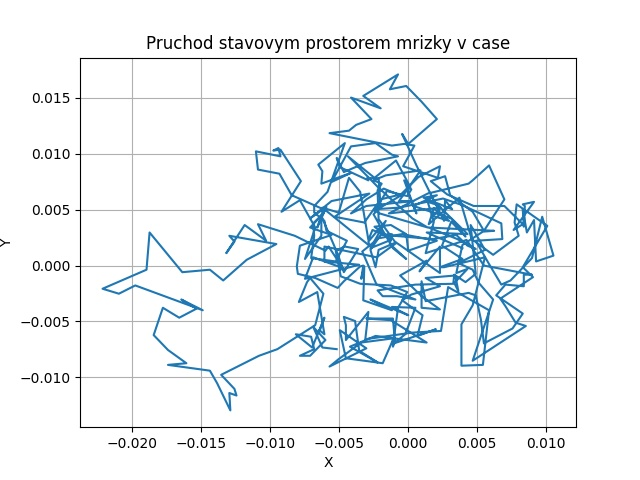
\includegraphics[scale=0.8]{cycle_a2b1}
 \caption{Cyklický diagram pro $\alpha=2, \beta=1$, kdy systém nevykazuje periodické chování. Body diagramu se nachází v blízkém okolí bodu $O$.}
\end{figure}

Pokud je $\beta$ zvoleno tak, že systém vykazuje periodické chování, nachází se v cyklických diagramech opravdu uzavřené křivky. Při menších $|\beta|$, s nižšími amplitudami středních hodnot v čase, křivky připomínají kružnici (viz Obrázek~\ref{fig:cycle_a2b3}), zatímco s rostoucím $|\beta|$ se křivky více podobají obdelníkům s oválnými vrcholy (viz Obrázek~\ref{fig:cycle_a2b6.75}).

Než se diagram ustálí na své charakteristické křivce, musí nejdřív přejít na vhodnou délku poloosy. Při tomto přechodu se v diagramu objevují spirálovité křivky.

\begin{figure}[H]
 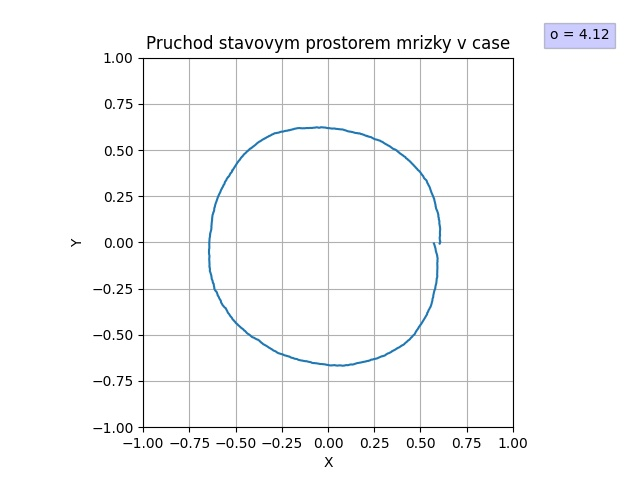
\includegraphics[scale=0.8]{cycle_a2b3}
 \caption{Cyklický diagram pro $\alpha=2, \beta=3$, kdy systém již částečně vykazuje periodické chování.}
 \label{fig:cycle_a2b3}
\end{figure}

\begin{figure}[H]
 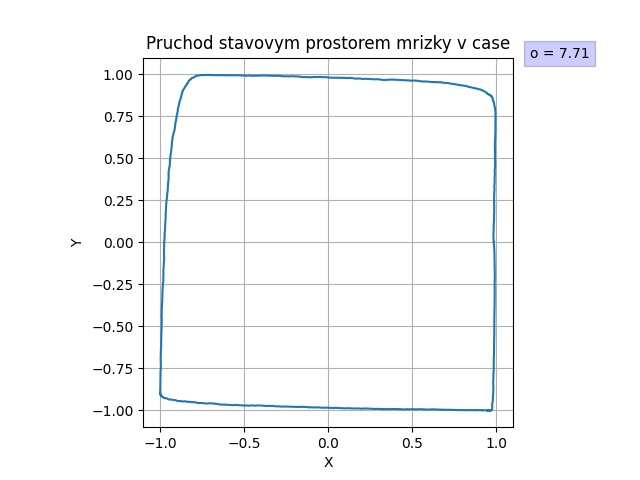
\includegraphics[scale=0.8]{cycle_a2b6.75}
 \caption{Cyklický diagram pro $\alpha=2, \beta=6.75$, kdy systém vykazuje plně periodické chování.}
 \label{fig:cycle_a2b6.75}
\end{figure}

Při $|\beta|$ dostatečně vysokém tak, že systém zmrzne (ve většině uzlů systém nabývá jedné hodnoty a nemění se), je v diagramu pouze množina bodů v okolí jednoho z bodů $(\pm 1, \pm 1)$. Není ale jisté, jestli v tomto okolí může systém setrvat, nebo jestli vždy po určité, dostatečně dlouhé době "přeskočí" a zamrzne v okolí jiného z extrémních bodů.

Pomocí cyklických diagramů můžeme systémům přiřadit další míry, které jsou závislé na parametrech $\alpha, \beta$. Tabulka obvodů diagramů v závislosti na parametrech vypadá takto:

\begin{center}
\begin{tabular}{ c|c|c}
 $\boldsymbol{\beta}$ & \textbf{a} & \textbf{o}\\
\hline
3.0 & 0.53 & 4.12 \\
3.25 & 0.67 & 5.03 \\
3.5 & 0.81 & 5.57 \\
3.75 & 0.85 & 5.91 \\
4.0 & 0.88 & 6.19 \\
4.25 & 0.9 & 6.36 \\
4.5 & 0.92 & 6.61 \\
4.75 & 0.93 & 6.76 \\
5.0 & 0.94 & 6.87 \\
5.25 & 0.95 & 7.05 \\
5.5 & 0.95 & 7.13 \\
5.75 & 0.96 & 7.26 \\
6.0 & 0.96 & 7.39 \\
6.25 & 0.96 & 7.53 \\
6.5 & 0.97 & 7.63 \\
6.75 & 0.98 & 7.71 \\
\end{tabular}
\end{center}
kde $o$ je obvod a $a = |OX|$, $O = (0,0)$, $X = (x, 0), x > 0$ (tedy jakási délka hlavní poloosy)


\subsection{Rovinná mřížka}
Na čtvercové mřížce se systém chová periodicky pouze lokálně, ale pro velká $L$ se přestávají jednotlivé uzly synchronizovat ve svém chování. 
\end{document} 
